\problemname{Amusement Park}
\begin{figure}[h]
    \centering
    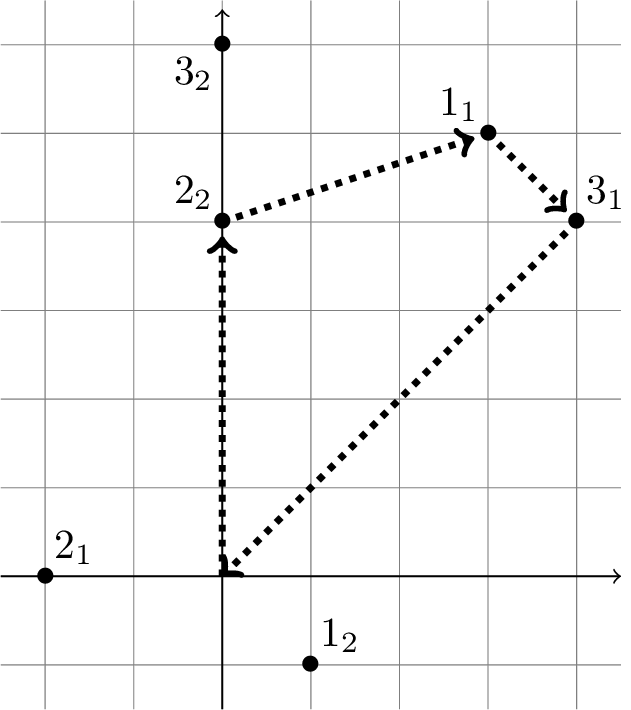
\includegraphics[width=0.2\textwidth]{tivoli}
    \caption{An illustration of the first sample with the optimal solution.}
\end{figure}
Lisa is visiting an amusement park and has decided which of the $N$ rides she wants to go on.
She wants to go on each ride exactly once.
For each ride, there are two equivalent facilities at different locations, i.e. $2N$ facilities in total.
Given the positions for each facility, help Lisa plan which facility to pick for each ride and in what order she should visit them to minimize the total distance she must walk to go on all the rides.
She starts and should finish at the entrance at $(0, 0)$.

\section*{Input}
The first line contains the integer $N$ ($1 \le N \le 15$), the number of rides Lisa wants to go on.
This is followed by $N$ lines, describing each ride.
One line contains four integers: the $x$ and $y$ coordinates of the first facility and then the $x$ and $y$ coordinates of the second facility.
The absolute value of each coordinate is less than a million.

No facility has a position coinciding with that of another or of the entrance.

\section*{Output}
The first line of the output should contain a decimal number: the minimum distance Lisa must walk.
Then print $N$ lines, each with two integers, listing the facilities she should visit.
The first integer on a line should be between $1$ and $N$ and denote the ride she goes to, while the second should be $1$ or $2$ and denote which of the two facilities she should choose.

If there are several paths that give the same distance, you can output any one of them.

The relative or absolute error may not exceed $10^{-5}$.

\section*{Scoring}
Your solution will be tested on a set of test case groups.
To get the points for a group, you need to pass all the test cases in the group.

\noindent
\begin{tabular}{| l | l | p{12cm} |}
  \hline
  \textbf{Group} & \textbf{Point value} & \textbf{Constraints} \\ \hline
  $1$    & $20$        & $N \le 1$ \\ \hline 
  $2$    & $40$        & $N \le 5$ \\ \hline
  $3$    & $40$        & No additional constraints. \\ \hline
\end{tabular}

